\chapter{Event Selection} \label{chapter:selection}

\section{Introduction}

    Run in parallel with the process of reconstruction, is that of event selection.
    As discussed earlier in Chapter \ref{chapter:trigger},
        there are far too many events in ATLAS to record and analyze them all.
    Thus, a series of selection algorithms are used to veto the abundance of background events.
    Unfortunately, these selection algorithms are not perfect,
        and so a careful balance must be achieved between removing a suitable amount of background,
        while retaining as many signal events as possible.

    \begin{figure}[tbh]
        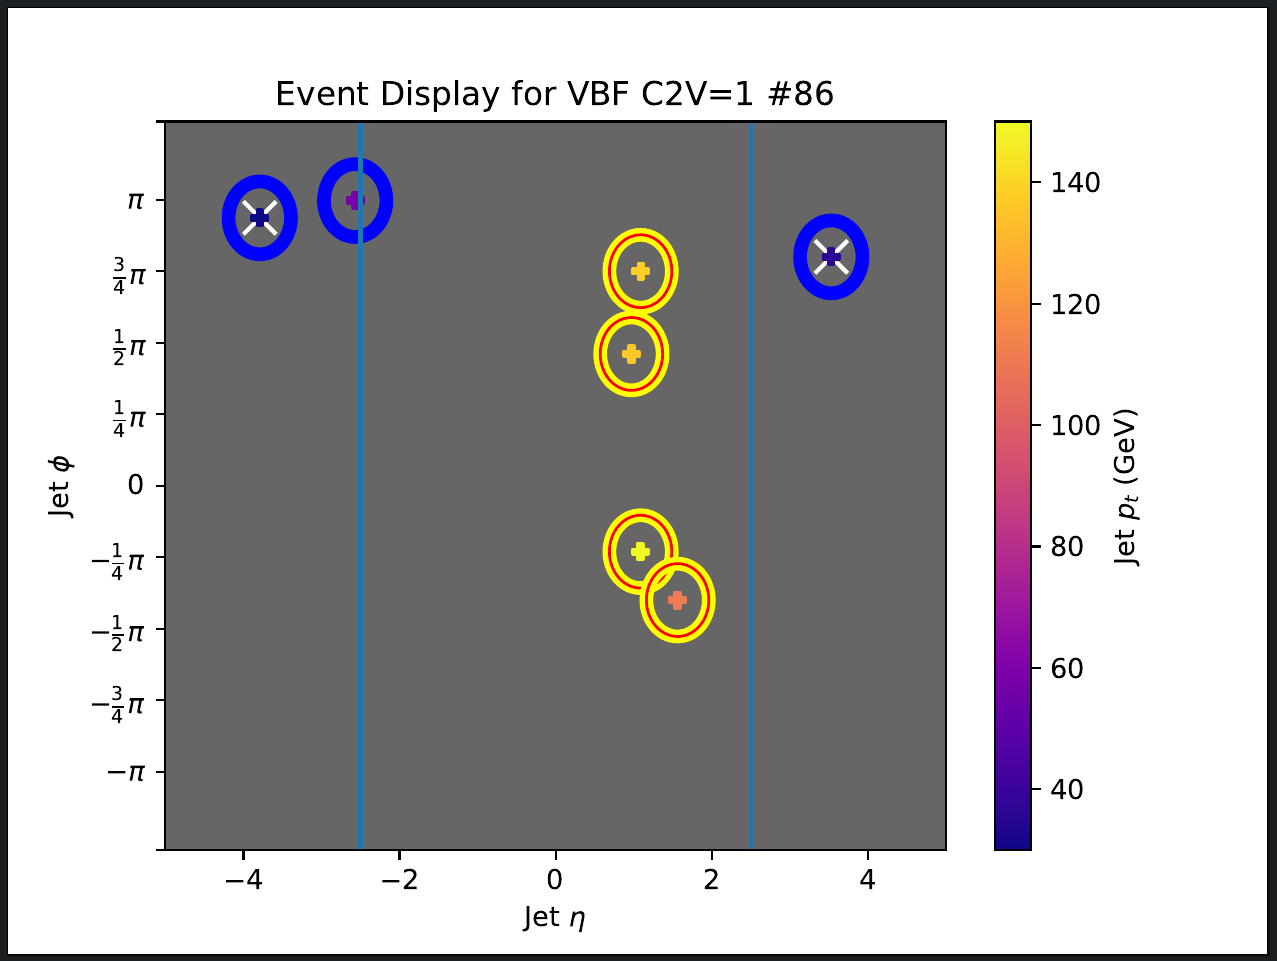
\includegraphics[width=\linewidth,height=\textheight,keepaspectratio]{selection/event_display}
        \caption{
            Event display of a typical VBF \to 4b event, visualized in $\eta-\phi$ space.
            The various circles correspond to jets in the event.
            The `+' sign in the center of every circle indicates the jet's $p_T$ (scale on right).
            The yellow circles correspond to the b-jet decay products of the Higgs bosons,
                and their red inlay indicates that they have been tagged as b-jets by the btagging algorithms.
            The blue jets with white `X's correspond to the VBF initial scatter jets.
            The final blue circle corresponds to a jet caused by a particle radiated by the nearby ID jet.
            The teal vertical lines designate $|\eta|=2.5$,
                the distinction between the ``Forward'' and ``Central'' regions.
        }
        \label{fig:event_display}
    \end{figure}

    %TODO also don't forget all the truth-level validation plots you have just LAYING AROUND ALREADY
    % that you can dump in here as a demonstration of probably any point you want to make
    
    Figure \ref{fig:event_display} is an ``event display'' of what a VBF \to 4b event is expected to look like,
        based on Monte-Carlo simulation (see Chapter \ref{chapter:signal}).
    It demonstrates the key features these selection algorithms use to differentiate signal from background.
    The most obvious feature to identify is the high-$p_T$-jet multiplicity.
    VBF \to 4b will, by definition, produce a total of six jets;
        the two initial-scatter (IS) light-quark jets, plus the 4 b-jets from the Higgs decay.
    All six of these jets will carry significant energy and transverse momentum.
    A hallmark of the VBF process is the wide opening angle and high invariant mass between the IS jets.
    Such a jet pattern stands out dramatically from most of the stochastic background noise,
        and is one of the main advantages of the VBF process.
    Additionally, while the four b-jets of the Higgs are not exclusively produced in the low-$\eta$ regions,
        so many high-$p_T$ b-jets orthogonal to the beamline is rare for background events,
        and thus makes for another highly identifiable feature of the signal.
    Finally, due to their high initial momentum,
        the $\bbar$ decay products of each Higgs will have little spread between them,
        producing an identifiable pattern in the final distribution of jets.

    All of these features are exploited by the selection process carried out in this analysis,
        which is performed across two distinct stages.
    The initial selection process is carried out before and during reconstruction, via the aforementioned trigger system.
    After the offline reconstruction process an additional set of selection criteria,
        specific to this analysis, are applied to the fully reconstructed event objects.
    
    \FloatBarrier
    \section{Triggers}
        
        The first stage of the Selection process largely occurs before reconstruction has even begun,
            in the L1, HLT, and Offline ATLAS Triggers.
        Table \ref{tab:nr-triggers-used} lists the trigger chains used in this analysis.
        An event from ATLAS is incorporated into the data used as long as it passes at least one 
            of the listed chains associated with its year.
        These triggers have been chosen based on any features that lend themselves to the VBF \to 4b process.
        Notably, the utilized triggers heavily emphasize high jet multiplicity and an abundance of b-jets.
        To understand how, it is necessary to understand the nomenclature of the trigger chains.
        A full reference can be found in [FIXME: find a reference for this],
            but a brief example of how to read the chains is provided here:

        HLT\_j110\_gsc150\_boffperf\_split\_2j45\_gsc55\_bmv2c1070\_split\_L1J85\_3J30:
        \begin{itemize}
            \item HLT: Most of the following requirements are based in the High Level Trigger
            \item j110: Requires one 110 GeV jet
            \item gsc150: Cut on jet $p_T \geq 150$ GeV after Global Sequential Calibration (GSC) algorithm is applied
            \item boffperf: b-jet Offline Performance algorithm
            \item split: Using ``Split'' track reconstruction algorithm
            \item 2j45: Find 2 jets with $p_T$ of at least 45 GeV
            \item gsc55: Cut on jet $p_T \geq 55$ GeV after GSC algorithm is applied
            \item bmv2c1070: passes b-jet MV2c10 algorithm at 70\% efficiency level
            \item split: (as above)
            \item L1J85: Level 1 Trigger algorithm requiring a cluster with an energy of at least 85 GeV 
            \item 3J30: Require at least 3 jets with a minimum $p_T$ of 30 GeV
        \end{itemize}
        [NOTE: the other reason I need to find a reference is to make sure I've got these right]


        % Triggers used in this analysis and why
        \begin{table}[htbp]
\centering \footnotesize
\begin{tabular}{ccc}
Year                      & Trigger Name                                                                    & \textbf{Trigger Type}  \\ 
\hline
\multirow{2}{*}{2016}                      & HLT\_j100\_2j55\_bmv2c2060\_split                                               & 2b1j                   \\
                      & HLT\_2j35\_bmv2c2060\_split\_2j35\_L14J15.0ETA25                                & 2b2j                   \\

\hline

\multirow{2}{*}{2017}                      & HLT\_j110\_gsc150\_boffperf\_split\_2j35\_gsc55\_bmv2c1070\_split\_L1J85\_3J30  & 2b1j                   \\
                      & HLT\_2j15\_gsc35\_bmv2c1040\_split\_2j15\_gsc35\_boffperf\_split\_L14J15.0ETA25 & 2b2j                   \\

\hline

\multirow{2}{*}{2018}                      & HLT\_j110\_gsc150\_boffperf\_split\_2j45\_gsc55\_bmv2c1070\_split\_L1J85\_3J30  & 2b1j                   \\
                      & HLT\_2j35\_bmv2c1060\_split\_2j35\_L14J15.0ETA25                                & 2b2j                   \\
                
\end{tabular}
\caption{Triggers used for non-resonant searches.\cite{hh4b_2021_int_note}}
\label{tab:nr-triggers-used}
\end{table}

        % (do we have any plots showing why we use these triggers?)
        %   Yes, though I might be able to get away without using them

        %Trigger bucketing strategy? What are the chances I can just not deal with this?


    \FloatBarrier
    \section{Analysis Cuts} \label{sec:analysis_cuts}

        Upon completion of the ATLAS-wide trigger selection,
            the appropriate data samples are copied for use by this analysis.
        The available data still contains a vast excess of background events though,
            and so this analysis makes an additional series of selection cuts on the fully reconstructed events.
        These cuts focus on the topological features discussed earlier,
            selecting events based on their jet multiplicity,
            the VBF jet kinematics,
            and the angular clustering of the Higgs decay products.

    \subsection{Jet Multiplicity and Categorization}
        
        First and foremost is a check to ensure that there are enough jets to even constitute a \vbfproc event.
        Moreover, the selection is particular about the quality and position of jets it will permit.
        Jets are categorized as ``Central'' if they fall within $|\eta| \leq 2.5$,
            and are ``Forward'' if they are found with $ 2.5 < |\eta| \leq 4.5 $.
        The reason for the distinction between the two is that Central jets fall within the boundaries of the ATLAS tracker system
            (see Section \ref{sec:inner_detector}).
        As the tracking system is necessary for the b-tagging algorithms,
            candidates for the Higgs' decay products are taken exclusively from Central jets.
        Central jets are only used if they have a $p_T > 40$ GeV, and satisfy at least one of the following three conditions:
            they pass the JVT algorithm, have $p_T > 60$ GeV, or have $2.4 < |\eta| < 2.5$.
        [TODO: I'm going to have to justify this wonky set of requirements huh?
            I haven't found a good explanation yet, so I might need to ask somebody
            (our int note just straight up skips these requirements, even though I can see them in the code)]
        Forward jets have less stringent requirements, needing only a $p_T > 30$ GeV.

        After jets have been categorized and selected, an event is only used if there at least six selected jets remaining.
        Of these, at least four must be Central jets which have been b-tagged by the trigger system.
        From the remaining jets (Central or Forward), there must be at least two \textit{anti}-b-tagged jets
            (i.e.\ jets that were marked as not b-jets).

        The VBF jets are chosen as the pair of anti-b-tagged jets with the largest vector-sum invariant mass ($m_{jj}$) between them,
            while the Higgs decay jets are chosen as the four highest-pt, b-tagged, Central jets.
        Any other jets in the event are discarded for the purposes of the rest of the analysis.
        The remaining selection cuts are made on these two categories of jets.
        
        %TODO: I should probably provide a source that justifies the mjj thing, since it's common practice
        % Maybe pull up one of the papers Ariel had you read?


    \subsection{VBF Topology}

        For the VBF jets, the charactistic wide-opening angle and high invariant mass is exploited here.
        The selected VBF pair must have a \deta between them of at least 3,
            and an mjj of at least 1 TeV.
        As well, the combined vector-sum-pt of all six jets
            (the four Higgs products and the two VBF jets)
            must be less than 65 GeV.
        The maximum sum-$p_T$ requirement follows from the fact that the initial incoming beamline particles have
            zero tranverse momentum, and so the output of their interaction should as well.
        These specfic values for the cuts are based on the significance values shown in Figure \ref{fig:vbf_cuts}).

        \begin{figure}[tbh]
            \subfloat[$m_{jj}$ Cut Significance]{
                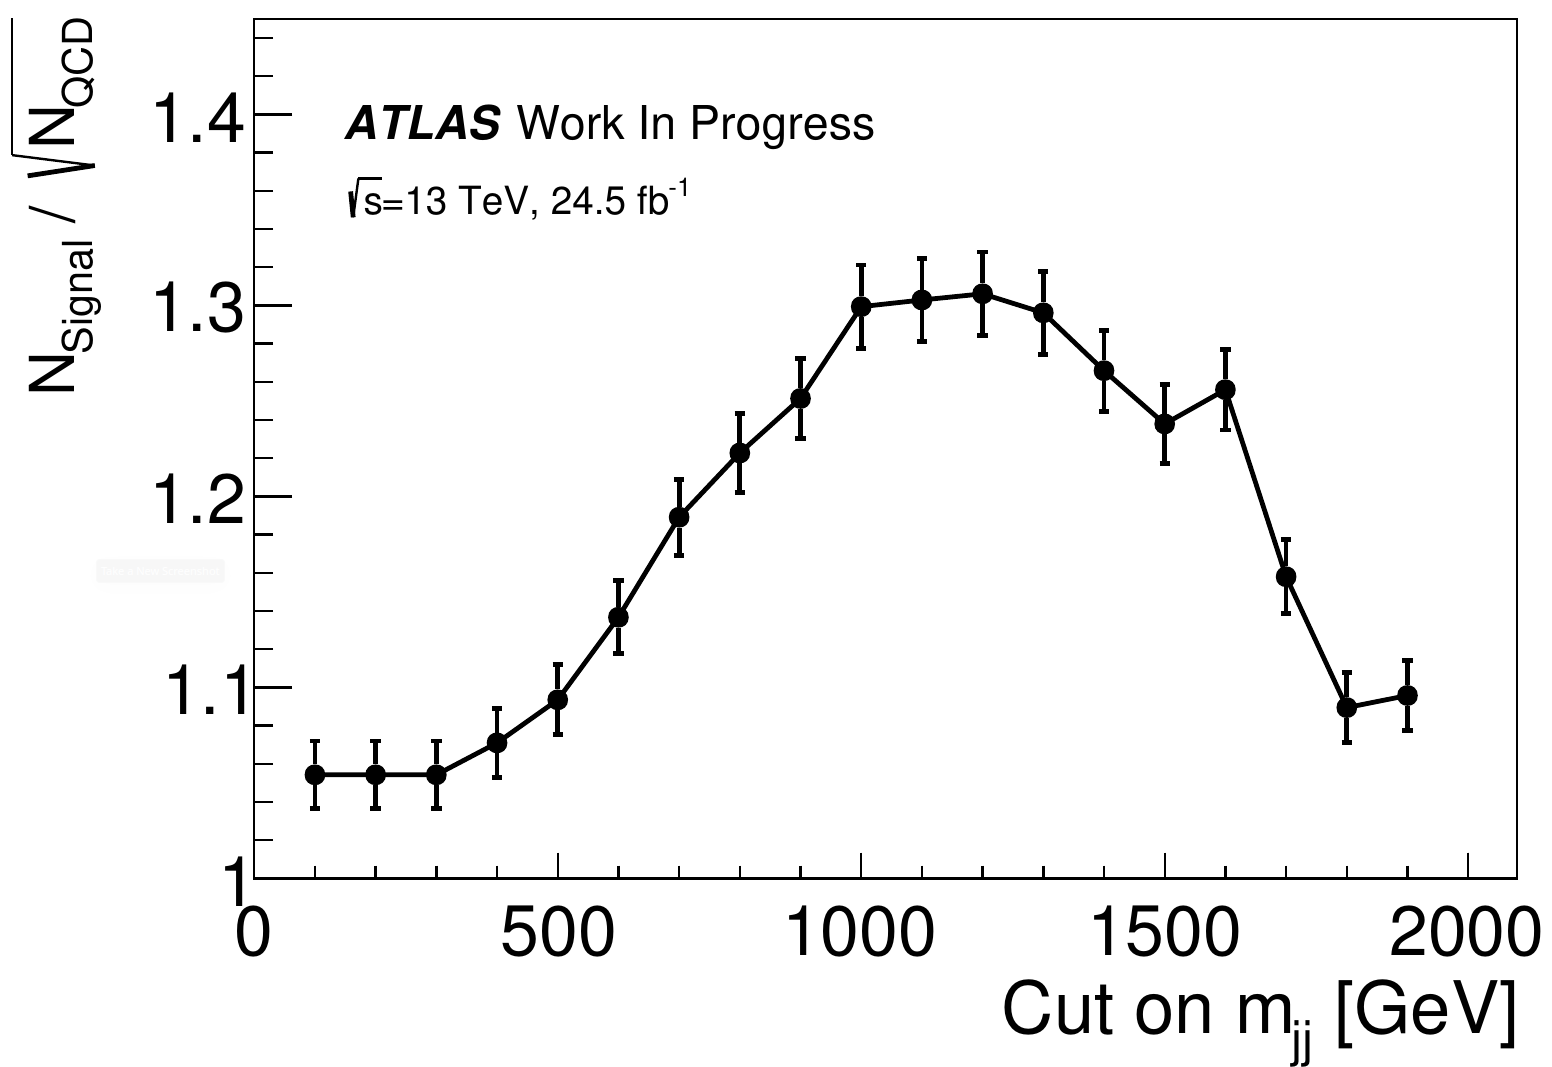
\includegraphics[width=0.5\linewidth,height=\textheight,keepaspectratio]{selection/mjj_significance}
            }
            \subfloat[$\deta_{jj}$ Cut Significance]{
                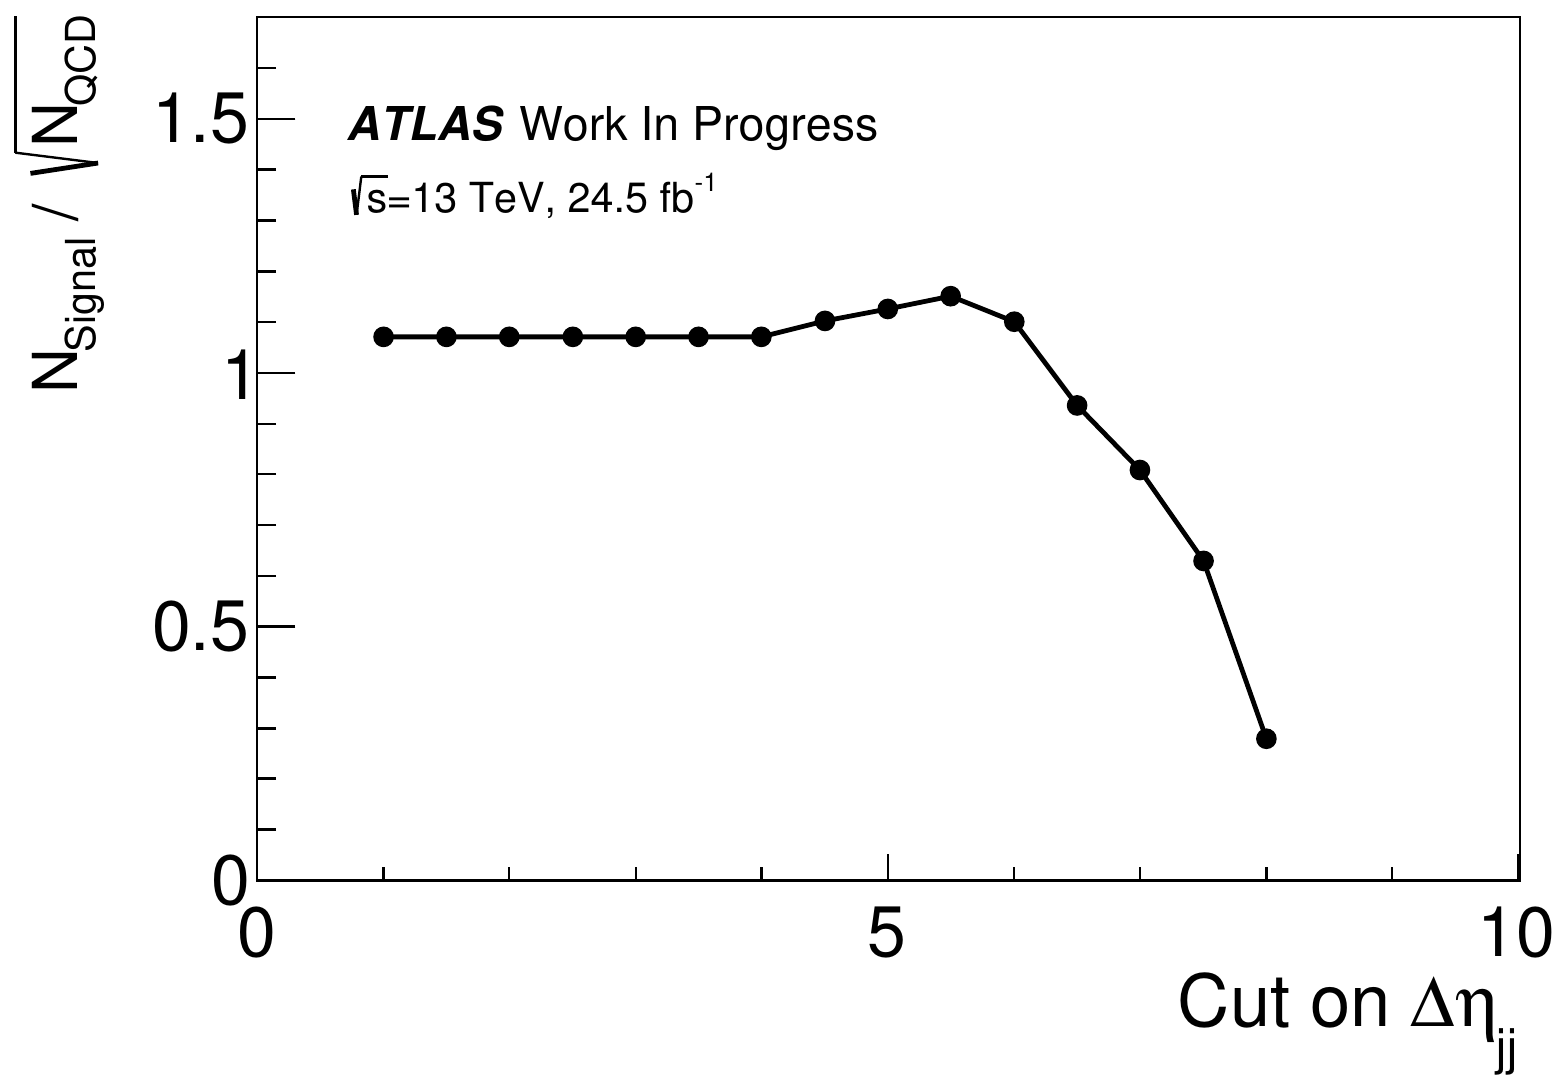
\includegraphics[width=0.5\linewidth,height=\textheight,keepaspectratio]{selection/detajj_significance}
            }\\
            \subfloat[6-Jet Vector-Sum $p_{T}$ Cut Significance]{
                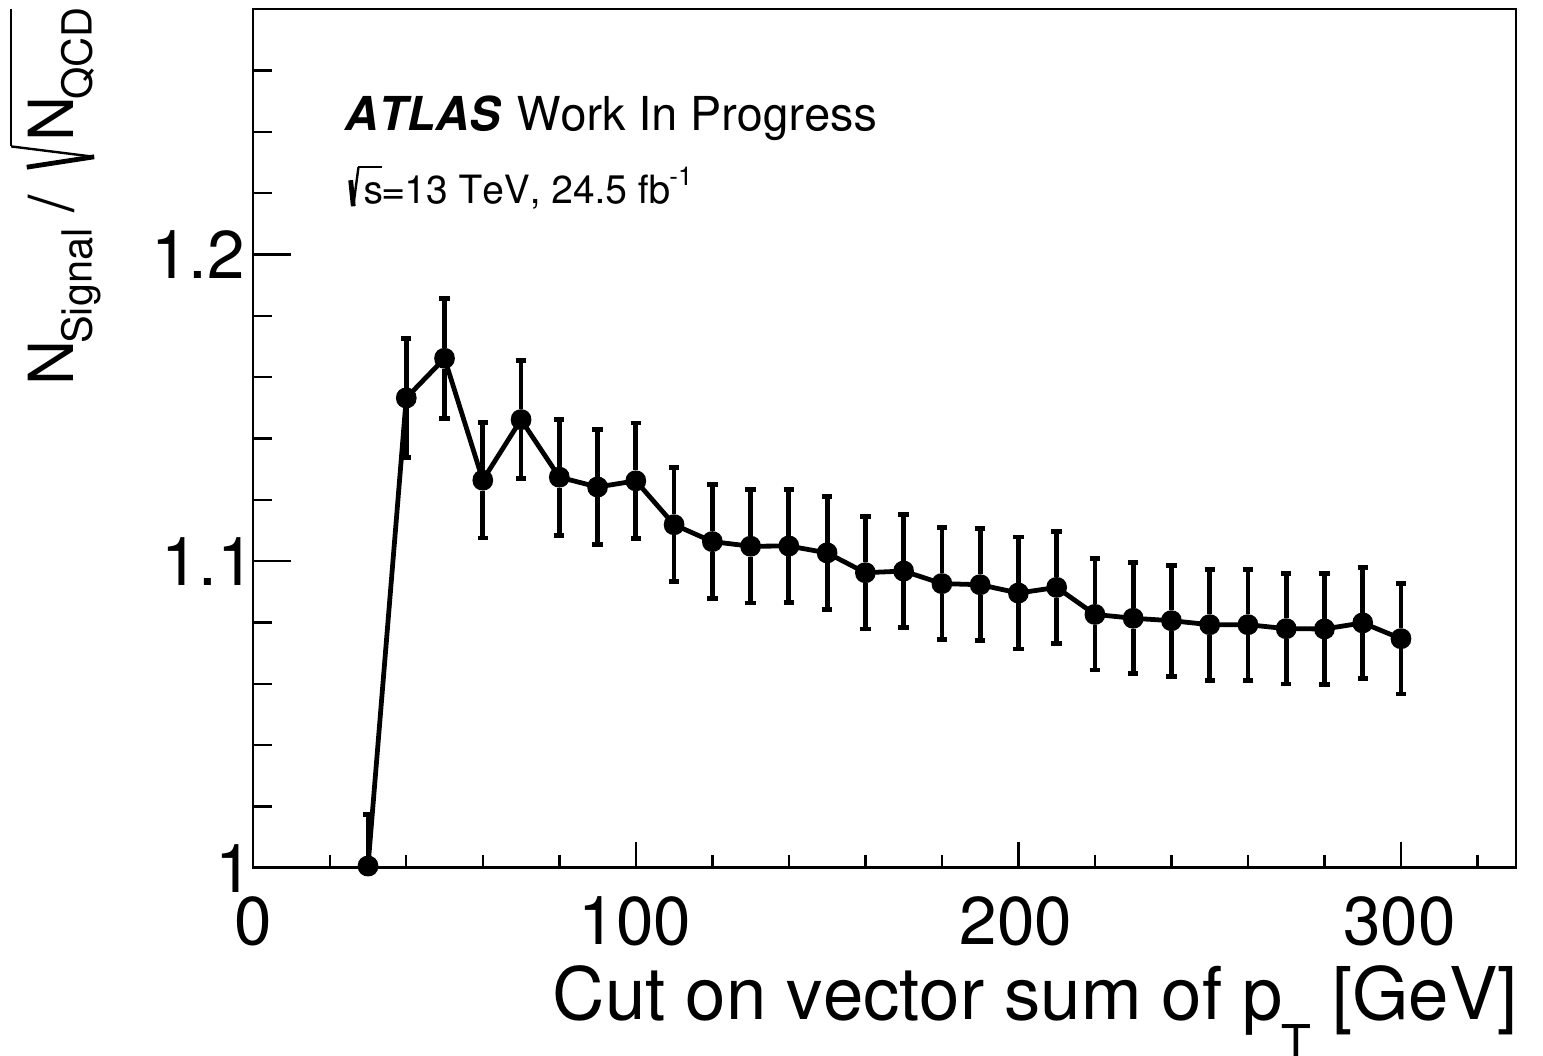
\includegraphics[width=0.5\linewidth,height=\textheight,keepaspectratio]{selection/vecsum_pt}
            }
            \caption{
                Significance value (see Chapter \ref{chapter:results})
                    for different cut values on the various VBF selection criteria\cite{vbf_hh_4b_2018_int}.
                TODO: I might need to replace these (especially the detajj one... that or our current cuts are super wrong).
            }
            \label{fig:vbf_cuts}
        \end{figure}
        \FloatBarrier


    \subsection{B-Quark Pairing}

        What is detected within ATLAS and reconstructed by Athena are not Higgs Bosons, but rather their decay products.
        To reconstruct the two Higgs Bosons, the four reconstructed b-quarks must be combined together, two b's to each Higgs.
        A pairing algorithm called MinDR\cite{hh4b_2021_int_note}
            is used to determine which b-quarks should be paired to each other.
        MinDR operates under the assumption that the decay products of the Higgs boson
            should be relatively close to each other in angular space, maintaining the Higgs' high $p_T$.
        With four jets, which need to be split into two pairs, there are three ways to choose the pairings.
        For each of the three pairing options, MinDR takes the pair with the leading $p_T$ as the ``leading Higgs Candidate''
        The pairing option which is chosen is that which minimizes the $\Delta R$ between the leading Higgs Candidate decay products
            (see Figure \ref{fig:minDR_pairing_diagram}).
        The effectiveness of this algorithm has been validated for multiple values of \kvv and \kl,
            as shown in Figure \ref{fig:HHpairing}.

        \begin{figure}[tbh]
            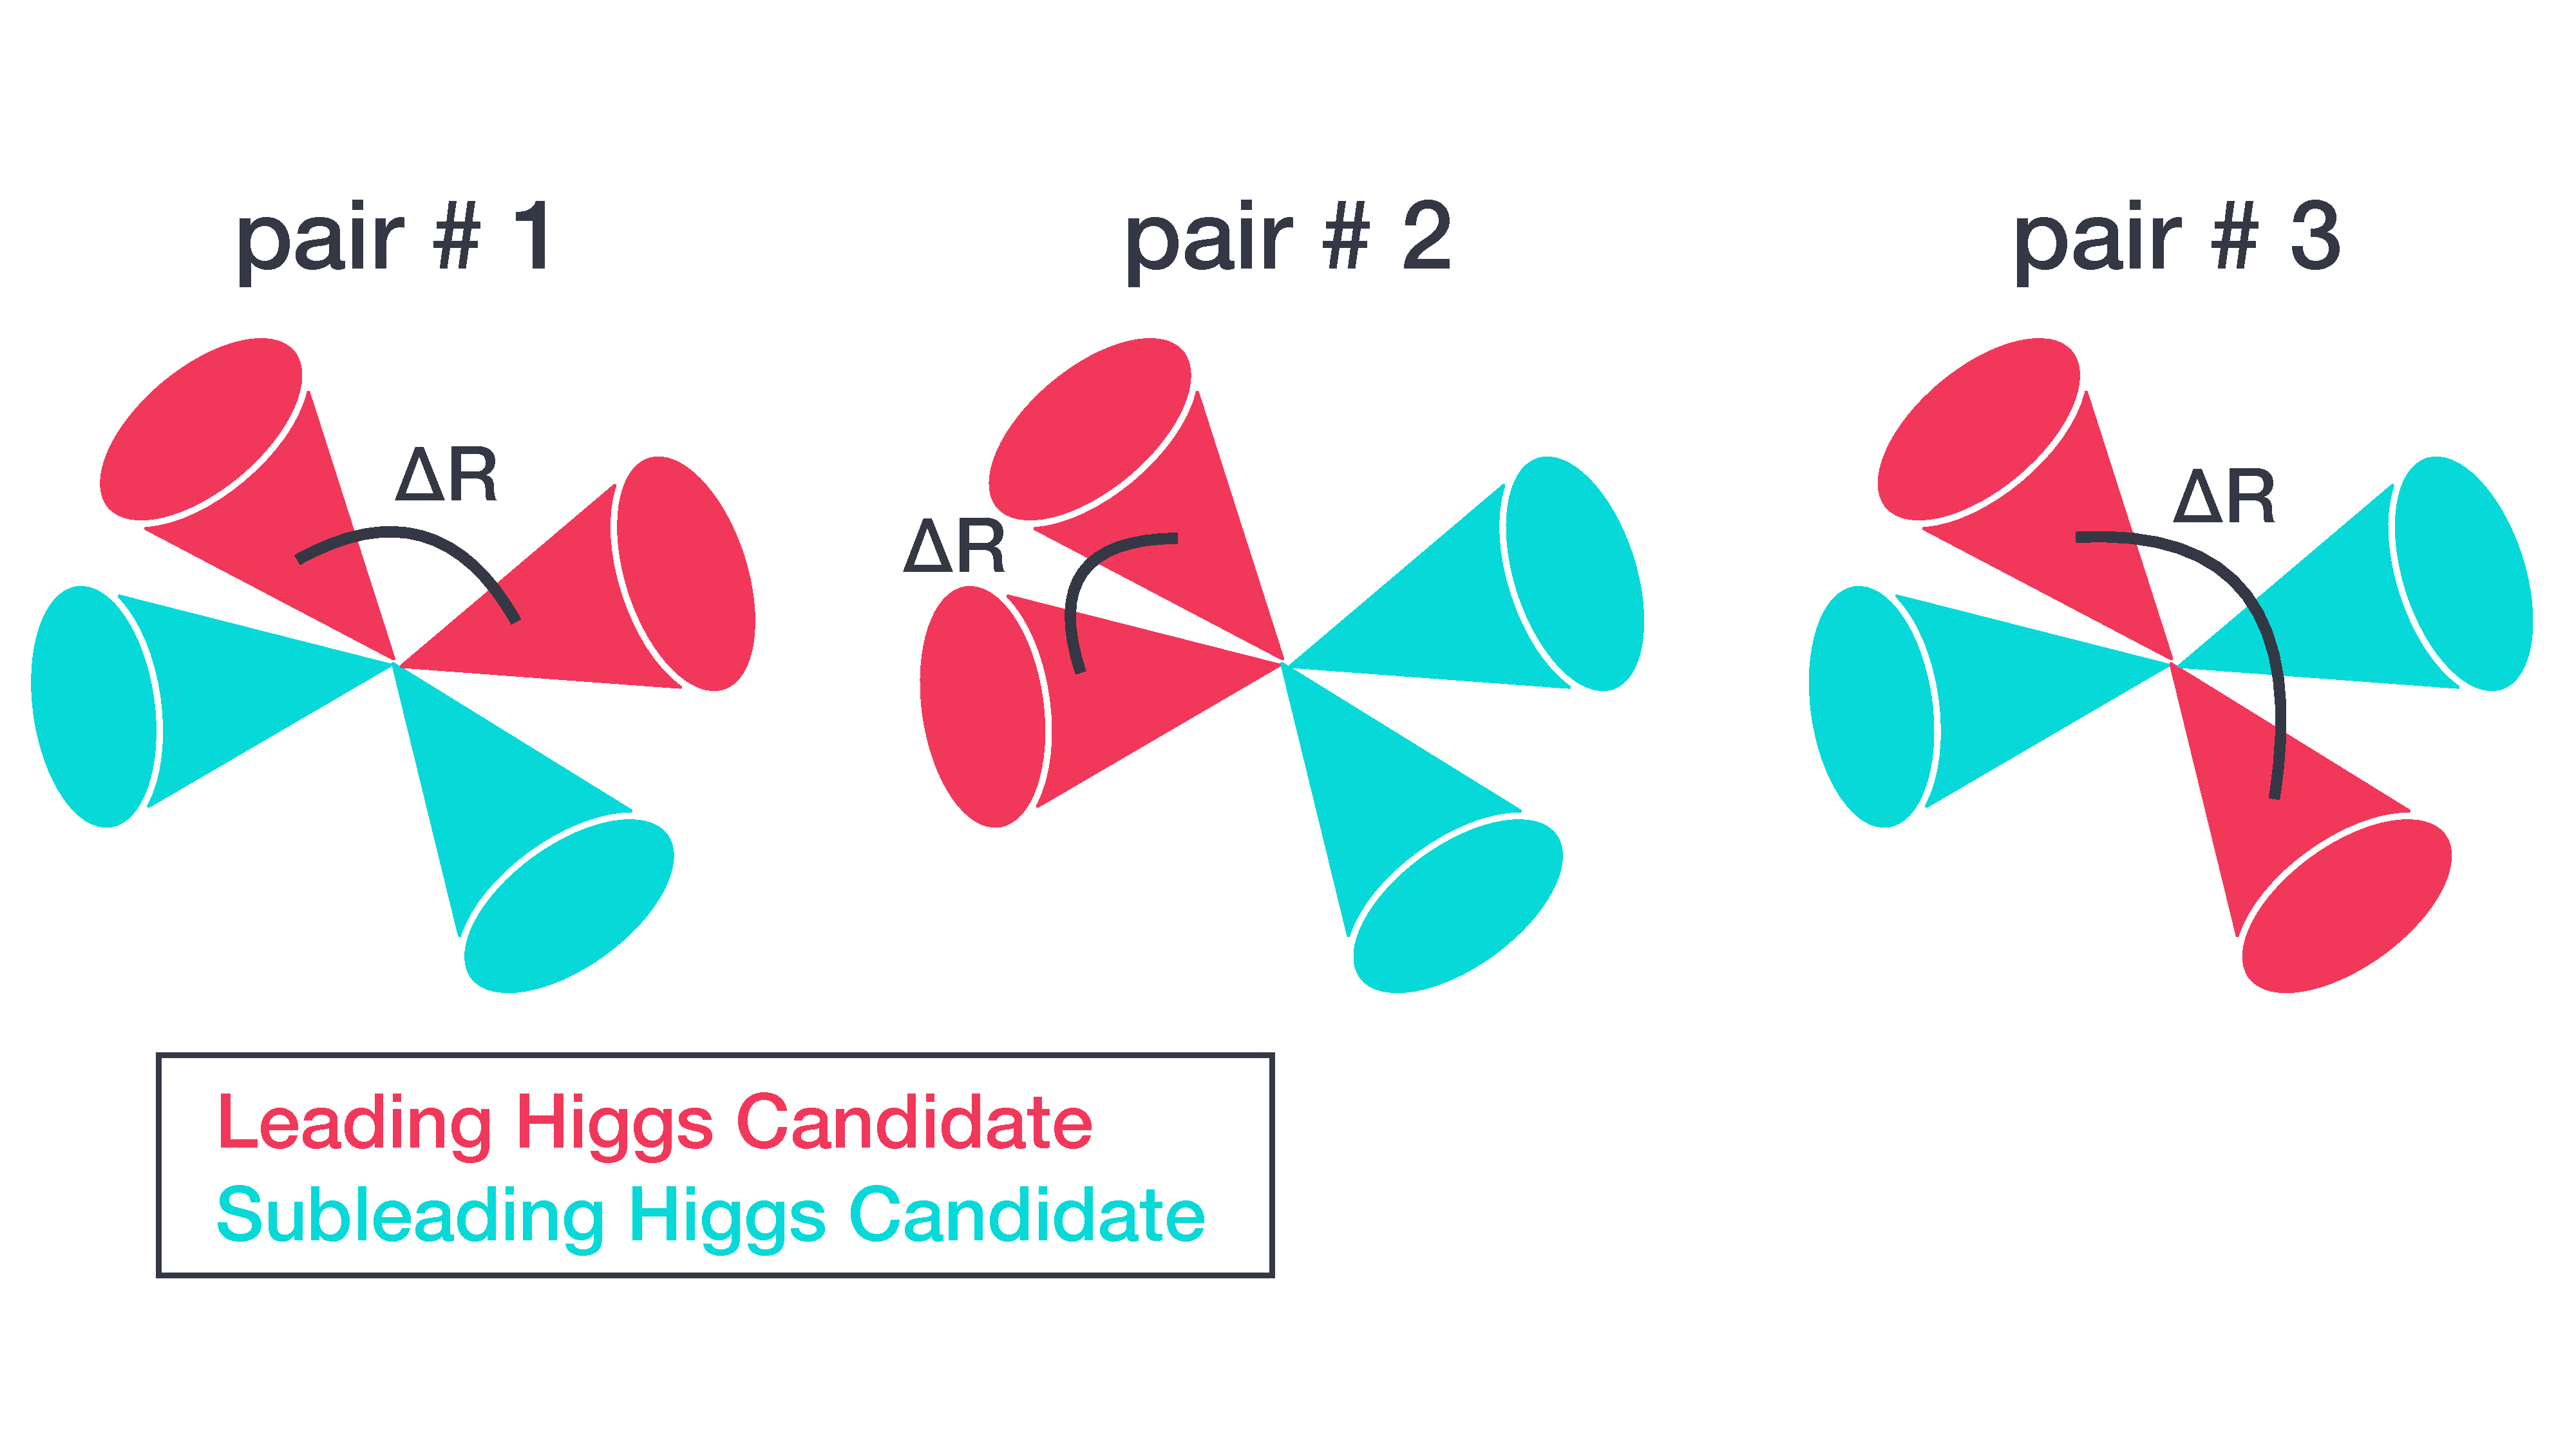
\includegraphics[width=\linewidth,height=\textheight,keepaspectratio]{selection/pairing}
            \caption{
                TODO (minDR picks pair 2 btw)\cite{hh4b_2021_int_note}
            }
            \label{fig:minDR_pairing_diagram}
        \end{figure}

        \begin{figure}[hbt]
            \centering
            \subfloat[Pairing accuracy vs \kl]{
                     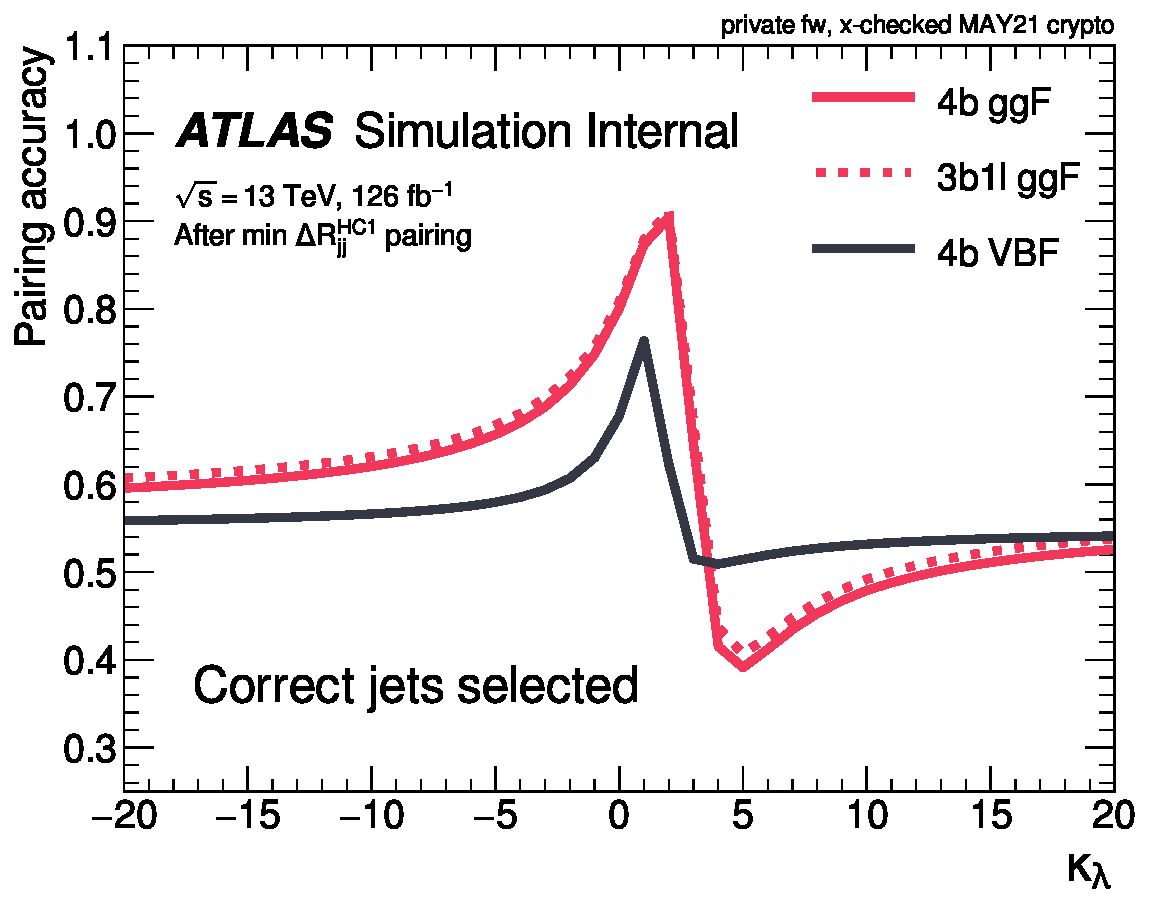
\includegraphics[width=0.4\textwidth]{selection/pairing_accuracy_kl}
                \label{fig:acc_kl_exists}
            }
            \subfloat[Pairing accuracy vs $\kappa_{2V}$]{
                     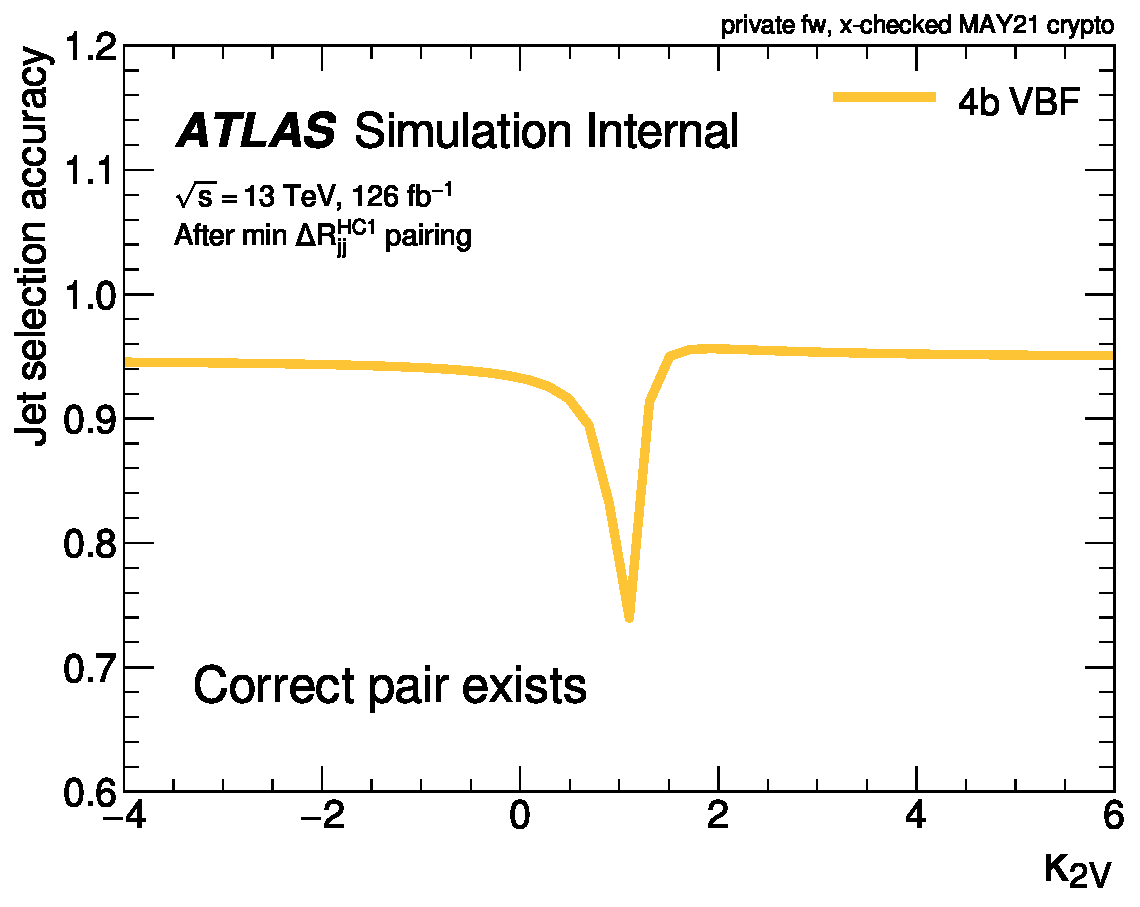
\includegraphics[width=0.4\textwidth]{selection/pairing_accuracy_k2v}
                \label{fig:acc_k2v_exists}
            }
            \caption{TODO \cite{hh4b_2021_int_note}}
            \label{fig:HHpairing}
        \end{figure}
                                                                                                         
        \FloatBarrier


    \subsection{Region Definition}
        
        There are three ``regions'' which are used for the analysis.
        Control Region 1 and 2 (CR1 and CR2) are used for the Background Estimation (see Chapter \ref{chapter:background}).
        The ``Signal'' Region is the set of data which will be used to search for the di-Higgs signal.

        Which region an event falls into is based on the reconstructed masses of the leading and sub-leading Higgs.
        The Signal Region (SR) corresponds to those events for which the reconstructed Higgs masses
            align closely with the measured value of the Higgs Boson (125 GeV), with additional room provided for error in measurment.
        CR1 and 2 are adjacent to the SR, designating events with kinematics very similar to the Signal Region,
            but with reconstructed Higgs masses incompatible with experimental measurment (see Figure \ref{fig:region_definition}).
        A quantity $X_{HH}$ governs the boundaries of these regions, and is defined as:

        \begin{equation}
            X_{HH} \equiv \sqrt{\left(\frac{m_{H1} - 124\textrm{GeV}}{0.1 \ m_{H1}}\right)^{2}
                + \left(\frac{m_{H2} - 117\textrm{GeV}}{0.1 \ m_{H2}}\right)^{2}}
            \label{eq:xhh}
        \end{equation}
        
        The SR is defined by $X_{hh} < 1.6$,
            while the CR and VR are set within a ring-like shape between the Signal Region
            and an outer bondary defined by:
        \begin{equation}
            \text{CR\ Outer\ Edge} \quad : \quad \sqrt{ \left(m_{H1} - 1.05 \cdot 124\textrm{GeV}\right)^2
                +  \left(m_{H2} - 1.05 \cdot 117\textrm{GeV}\right)^2 } = 45\textrm{GeV}
            \label{eq:cr_out}
        \end{equation}
        
        The split between the CR and VR is based on studies demonstrating that this split results in
            close kinematic similarity between the two regions.
        With the final set of data samples selected and placed into the required subsets, 
            the process of analyzing the data can begin.

        \begin{figure}[tbh]
            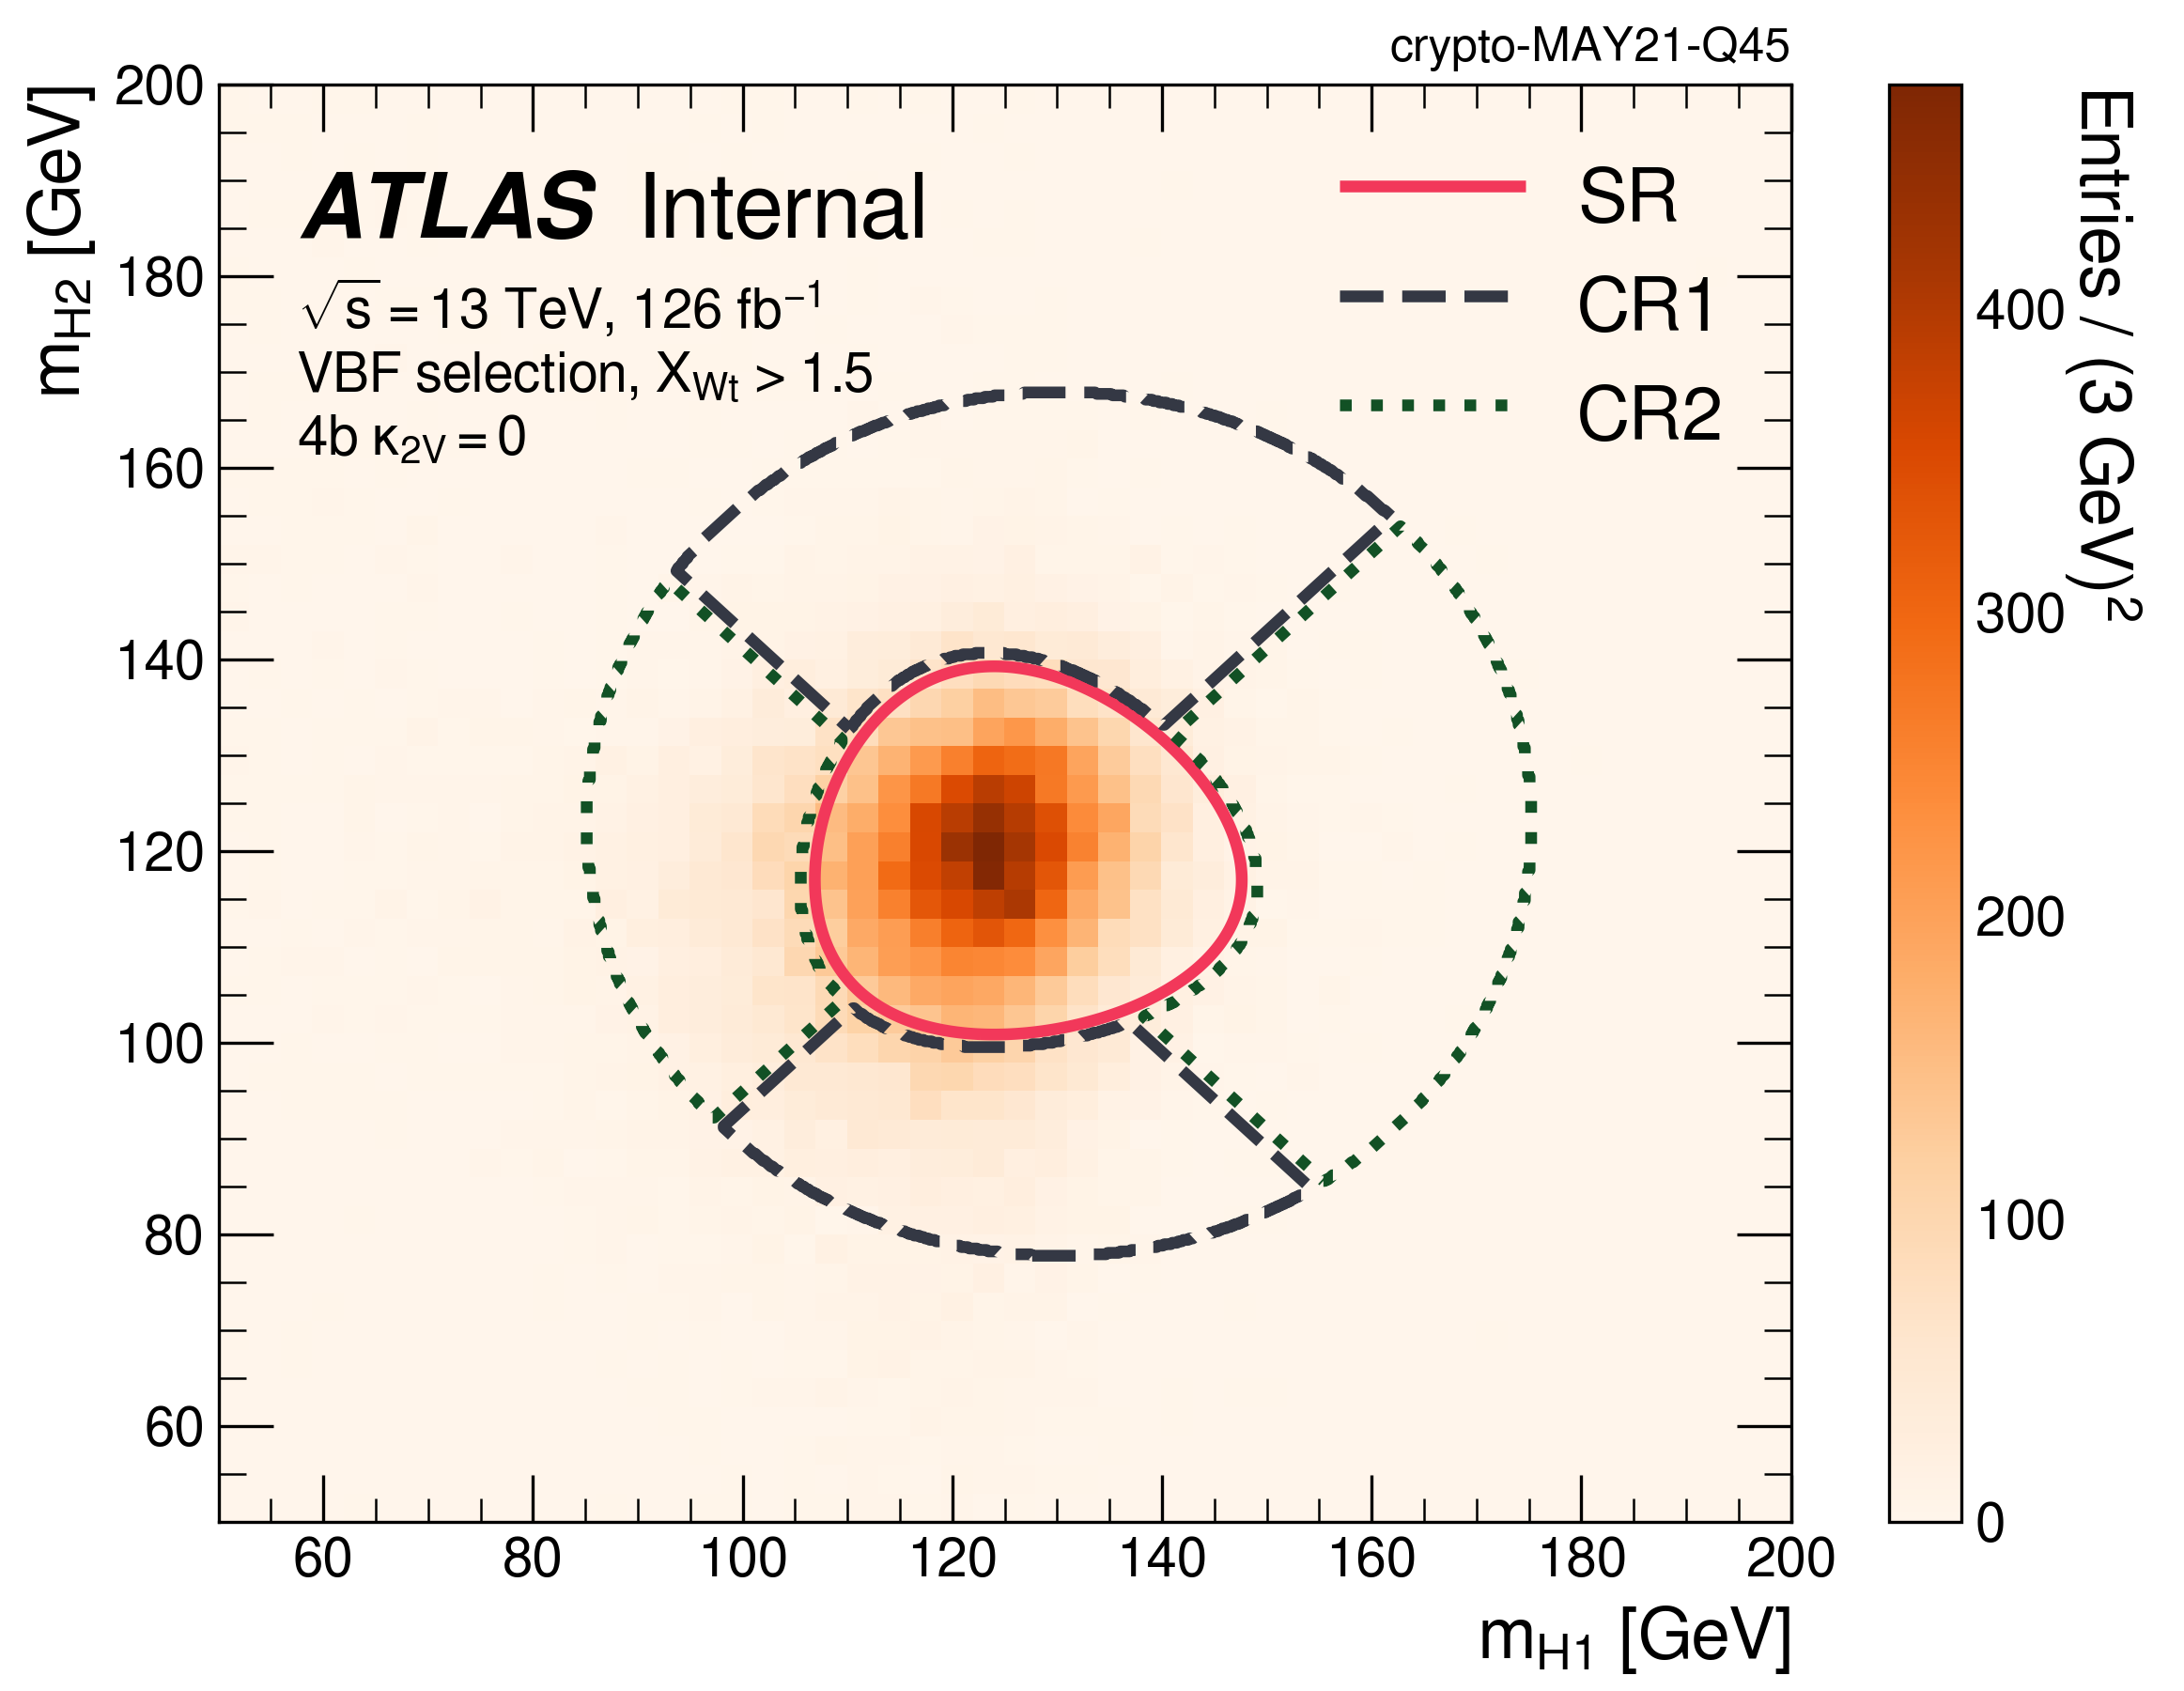
\includegraphics[width=\linewidth,height=\textheight,keepaspectratio]{selection/massplane_sig_all_4b_vbf_Xwt_1p5_k2V_0}
            \caption{
                TODO, We use k2v=0 because we're trying to exclude it.\cite{hh4b_2021_int_note}
            }
            \label{fig:region_definition}
        \end{figure}
